\section{Interfaccia di monitoraggio}
Durante lo sviluppo del progetto è stato sviluppato in parallelo un semplice \textbf{sistema di monitoring} informazioni riguardo le simulazioni eseguite ed i server slave collegati. In particolare è stato utilizzato il linguaggio \textbf{TypeScript}, con il framework \textbf{Angular}. Vengono utilizati i dati forniti dalla \textbf{REST API} implementata all'interno dell'esempio di avvio del progetto del server master.

Il codice del frontend è contenuto all'interno di una apposita \href{https://github.com/ZamponiMarco/sibilla-frontend}{\textbf{repository in GitHub}}. Per avviare il progetto bisogna eseguire il \textbf{clone della repository} ed eseguire il comando \texttt{ng serve} all'interno della cartella di root del progetto. Il frontend richiede che \textbf{node.js} e il pacchetto npm \textbf{@angular-cli} siano installati nel sistema.

\begin{figure}[H]
    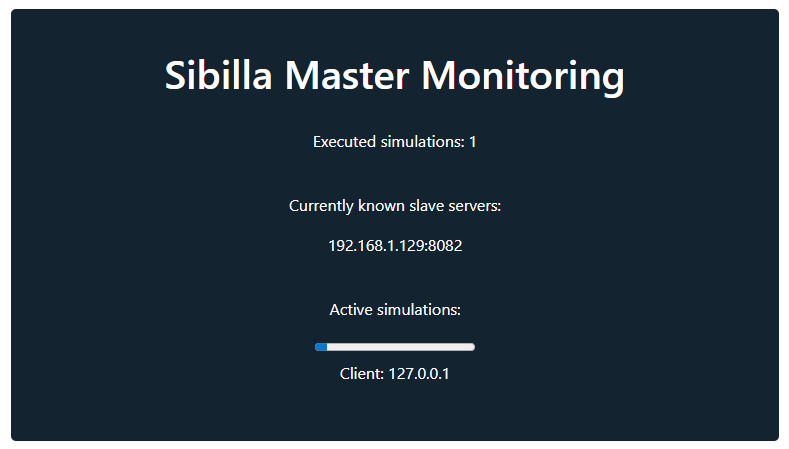
\includegraphics[width=\linewidth]{images/monitoring_frontend.PNG}
    \captionsetup{justification=centering}
    \caption{Una schermata del frontend che monitora un master server}
\end{figure}